\documentclass[12pt,a4paper]{article}

% ── Packages ──────────────────────────────────────────────────────
\usepackage[margin=2.5cm]{geometry}
\usepackage{graphicx}
\usepackage{float}
\usepackage{booktabs}
\usepackage{longtable}
\usepackage{array}
\usepackage{xcolor}
\usepackage{listings}
\usepackage{hyperref}
\usepackage{titlesec}
\usepackage{fancyhdr}
\usepackage{amsmath}
\usepackage{caption}
\usepackage{subcaption}
\usepackage{enumitem}
\usepackage{tikz}
\usepackage{pgfplots}
\pgfplotsset{compat=1.18}
\usepackage{mdframed}
\usepackage{tcolorbox}
\usepackage{parskip}
%\usepackage{microtype}

% ── Colors ─────────────────────────────────────────────────────────
\definecolor{carbonbg}{HTML}{13141a}
\definecolor{primary}{HTML}{4f8ef7}
\definecolor{accent}{HTML}{00d4aa}
\definecolor{danger}{HTML}{ff5c6a}
\definecolor{muted}{HTML}{9ba3be}
\definecolor{codebg}{HTML}{1c1e2a}
\definecolor{codefg}{HTML}{e8eaf0}

% ── Hyperref Setup ─────────────────────────────────────────────────
\hypersetup{
    colorlinks=true,
    linkcolor=primary,
    urlcolor=accent,
    pdftitle={SortLab - Sorting Algorithm Analyser Report},
    pdfauthor={Eyad Amr}
}

% ── Code Listing Style ─────────────────────────────────────────────
\lstdefinestyle{javastyle}{
    backgroundcolor=\color{codebg},
    basicstyle=\ttfamily\footnotesize\color{codefg},
    keywordstyle=\color{primary},
    commentstyle=\color{muted}\itshape,
    stringstyle=\color{accent},
    numberstyle=\tiny\color{muted},
    breaklines=true,
    frame=single,
    rulecolor=\color{muted},
    numbers=left,
    tabsize=4,
    showstringspaces=false,
    language=Java,
    captionpos=b
}

\lstdefinestyle{pythonstyle}{
    backgroundcolor=\color{codebg},
    basicstyle=\ttfamily\footnotesize\color{codefg},
    keywordstyle=\color{primary},
    commentstyle=\color{muted}\itshape,
    stringstyle=\color{accent},
    numberstyle=\tiny\color{muted},
    breaklines=true,
    frame=single,
    rulecolor=\color{muted},
    numbers=left,
    tabsize=4,
    showstringspaces=false,
    language=Python,
    captionpos=b
}

\lstset{style=javastyle}

% ── Section Title Formatting ───────────────────────────────────────
\titleformat{\section}
  {\Large\bfseries\color{primary}}
  {\thesection}{1em}{}[\titlerule]

\titleformat{\subsection}
  {\large\bfseries\color{primary!80!black}}
  {\thesubsection}{1em}{}

\titleformat{\subsubsection}
  {\normalsize\bfseries\color{muted}}
  {\thesubsubsection}{1em}{}

% ── Header / Footer ────────────────────────────────────────────────
\pagestyle{fancy}
\fancyhf{}
\fancyhead[L]{\small\textcolor{muted}{SortLab — Algorithm Analyser}}
\fancyhead[R]{\small\textcolor{muted}{Eyad Amr}}
\fancyfoot[C]{\small\textcolor{muted}{\thepage}}
\renewcommand{\headrulewidth}{0.4pt}
\renewcommand{\headrule}{\hbox to\headwidth{\color{muted}\leaders\hrule height \headrulewidth\hfill}}

% ── Infobox ────────────────────────────────────────────────────────
\newtcolorbox{infobox}[1][]{
  colback=codebg!10,
  colframe=primary,
  coltitle=white,
  fonttitle=\bfseries,
  boxrule=0.5pt,
  arc=4pt,
  left=8pt, right=8pt, top=6pt, bottom=6pt,
  #1
}

\newtcolorbox{designbox}[1][]{
  colback=accent!5,
  colframe=accent,
  coltitle=white,
  fonttitle=\bfseries,
  boxrule=0.5pt,
  arc=4pt,
  left=8pt, right=8pt, top=6pt, bottom=6pt,
  #1
}

\newtcolorbox{notebox}[1][]{
  colback=danger!5,
  colframe=danger,
  boxrule=0.5pt,
  arc=4pt,
  left=8pt, right=8pt, top=6pt, bottom=6pt,
  #1
}

% ══════════════════════════════════════════════════════════════════
\begin{document}
% ══════════════════════════════════════════════════════════════════

% ── Title Page ─────────────────────────────────────────────────────
\begin{titlepage}
    \centering
    \vspace*{2cm}

    {\Huge\bfseries\color{primary} Sorting Algorithm Lab}\\[0.5em]
    {\Large\color{muted} Sorting Algorithm Analyser \& Visualiser}\\[3em]

    \rule{\textwidth}{0.5pt}\\[1em]
    {\large\bfseries Project Report}\\[0.5em]
    {\normalsize Data Structures \& Algorithms}\\
    \rule{\textwidth}{0.5pt}\\[3em]

    {\large\textbf{Eyad Amr Asaad}}\\[0.5em]
     {\large\textbf{23010312}}\\[0.5em]
    {\color{muted} Computer Engineering Departement}\\[3em]

    \vfill

    \begin{infobox}[title=Project Summary]
        Sorting Algorithm Lab is a JavaFX desktop application that enables users to benchmark,
        compare, and visually animate six classic sorting algorithms in real time.
        The system supports randomised and file-based input, parallel execution,
        CSV export, and a Python-powered statistical analysis suite.
    \end{infobox}

    \vspace{2em}
    {\color{muted}\today}
\end{titlepage}

% ── Table of Contents ──────────────────────────────────────────────
\tableofcontents
\newpage

% ══════════════════════════════════════════════════════════════════
\section{Introduction}
% ══════════════════════════════════════════════════════════════════

SortLab is a full-featured desktop application built with Java 21 and JavaFX 21
that provides two complementary modes for studying sorting algorithms:
\textbf{Comparison Mode} and \textbf{Visualization Mode}. The application was
designed with the goal of making algorithm analysis both rigorous and intuitive —
allowing a user to benchmark algorithms with thousands of runs in one tab, and
then watch the same algorithms animate bar-by-bar in another.

The six algorithms implemented are:

\begin{center}
\begin{tabular}{lll}
\toprule
\textbf{Algorithm} & \textbf{Best Case} & \textbf{Worst Case} \\
\midrule
Bubble Sort    & $O(n)$        & $O(n^2)$       \\
Insertion Sort & $O(n)$        & $O(n^2)$       \\
Selection Sort & $O(n^2)$      & $O(n^2)$       \\
Merge Sort     & $O(n \log n)$ & $O(n \log n)$  \\
Quick Sort     & $O(n \log n)$ & $O(n^2)$       \\
Heap Sort      & $O(n \log n)$ & $O(n \log n)$  \\
\bottomrule
\end{tabular}
\end{center}

The project is built on Maven and follows a clean layered architecture separating
algorithm logic, data models, comparison infrastructure, visualisation rendering,
and the UI controller layer.

% ══════════════════════════════════════════════════════════════════
\section{Design \& Architecture}
% ══════════════════════════════════════════════════════════════════

\subsection{High-Level Architecture}

The application is structured into five distinct packages, each with a clearly
defined responsibility:

\begin{center}
\begin{tabular}{ll}
\toprule
\textbf{Package} & \textbf{Responsibility} \\
\midrule
\texttt{sorting.algorithms}  & All six sort implementations + interface/factory \\
\texttt{sorting.model}       & Data transfer objects (task, result, summary, step) \\
\texttt{sorting.comparison}  & Benchmark runner, parallel manager, CSV export \\
\texttt{sorting.visualization} & Canvas rendering, animation engine, audio feedback \\
\texttt{sorting.ui}          & JavaFX controllers for both application tabs \\
\texttt{sorting.input}       & Array generation from random or file input \\
\midrule
\texttt{resources/fxml}      & FXML layout files (Main, Comparison, Visualization) \\
\texttt{resources/css}       & Carbon Dark stylesheet \\
\bottomrule
\end{tabular}
\end{center}

\begin{figure}[H]
    \centering
    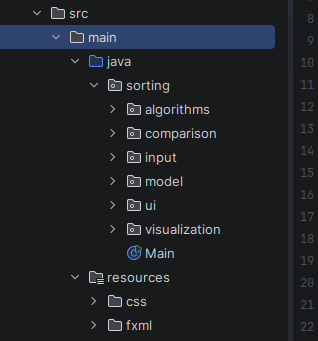
\includegraphics[width=\linewidth]{Images/Structure.png}
    \caption{Caption here}
\end{figure}

\subsection{Key Design Decisions}

\subsubsection{Strategy Pattern via \texttt{SortAlgorithm} Interface}

Every sorting algorithm implements the \texttt{SortAlgorithm} interface:

\begin{lstlisting}[caption={SortAlgorithm interface}]
public interface SortAlgorithm {
    void sort(int[] array);
    String getName();
    long getComparisons();
    long getInterchanges();
    void reset();
    List<SortStep> getSteps();
    void setSteps(boolean collectSteps);
}
\end{lstlisting}

This means the rest of the application never references a concrete class
(e.g.\ \texttt{BubbleSort}) directly. Instead, the \texttt{SortAlgorithmFactory}
instantiates the right implementation from a string name, and all callers work
against the interface. Adding a seventh algorithm in the future requires only
two changes: write the class, and add one line to the factory.

\subsubsection{\texttt{AbstractSort} — Shared State \& Helpers}

All six algorithms extend \texttt{AbstractSort}, which holds shared state
(\texttt{comparisons}, \texttt{interchanges}, \texttt{steps}), and provides
protected helpers:

\begin{itemize}[nosep]
    \item \texttt{swap(array, i, j)} — performs the swap and is the single
          point where interchanges should be counted.
    \item \texttt{addStep(array, activeIndex)} — clones the current array state
          into a \texttt{SortStep} only when \texttt{collectSteps = true},
          keeping benchmarking fast (no step collection overhead).
    \item \texttt{reset()} — clears all counters and the steps list so the
          same instance can be reused across runs.
\end{itemize}

\subsubsection{Fair Comparison via a Shared Base Array}

In Visualization Mode, all selected algorithms receive an identical clone of the
same randomly generated base array. This is a deliberate design decision: if
each algorithm were given a different random array, the comparison would be
meaningless because one algorithm might simply have received an easier input.

\begin{designbox}[title=Why This Matters]
    QuickSort is sensitive to input distribution. Given a sorted array it
    degrades to $O(n^2)$. By sharing one base array, both QuickSort and
    BubbleSort are always racing on the same problem instance, making runtime
    differences attributable entirely to algorithm efficiency rather than luck.
\end{designbox}

\subsubsection{Dual-Mode Step Collection}

The \texttt{setSteps(boolean)} flag on \texttt{AbstractSort} controls whether
sorting steps are recorded. In Comparison Mode this flag is \texttt{false}, so
sorts run at full speed without the memory overhead of storing thousands of array
snapshots. In Visualization Mode it is set to \texttt{true} so the
\texttt{SortAnimator} can play them back frame-by-frame.

\subsubsection{File Input Support}

Both modes accept integer arrays from plain text files (e.g.\ \texttt{[5, 1, 2, 6, 4]}
on a single line). \texttt{ArrayGenerator.generateFromFile(String fullPath)}
accepts the absolute path returned directly by JavaFX's \texttt{FileChooser}, so
no path manipulation is needed. Comparison Mode supports multi-file selection
(\texttt{showOpenMultipleDialog}), creating one task per file per algorithm.
Visualization Mode uses single-file selection (\texttt{showOpenDialog}).

% ══════════════════════════════════════════════════════════════════
\section{Algorithm Implementations}
% ══════════════════════════════════════════════════════════════════

\subsection{Bubble Sort}

Bubble Sort makes repeated passes over the array, comparing adjacent elements
and swapping them if they are in the wrong order. After each pass the largest
unsorted element ``bubbles'' to its correct position. The outer loop shrinks
the unsorted region by one element each pass.

\begin{itemize}[nosep]
    \item \textbf{Comparisons counted:} after every adjacent pair comparison.
    \item \textbf{Interchanges counted:} every time a swap is performed.
    \item \textbf{Steps added:} before the comparison and after every swap.
\end{itemize}

\textbf{Complexity:} $O(n^2)$ time, $O(1)$ space.

\subsection{Insertion Sort}

Insertion Sort builds a sorted prefix from left to right. For each element
\texttt{array[i]}, it is saved in \texttt{temp} and the inner \texttt{while}
loop shifts elements right until the correct insertion position is found.

\begin{itemize}[nosep]
    \item \textbf{Notable implementation detail:} shifting elements right
          (\texttt{array[j+1] = array[j]}) counts as an interchange.
    \item Performs very well on nearly-sorted data because the inner loop
          exits early.
\end{itemize}

\textbf{Complexity:} $O(n^2)$ worst, $O(n)$ best, $O(1)$ space.

\subsection{Selection Sort}

Selection Sort finds the minimum of the unsorted suffix and swaps it into the
current position. It is unique in making exactly $n-1$ swaps regardless of
input, which is why Interchanges stays very low in the analysis charts.

\begin{itemize}[nosep]
    \item \textbf{Always} $\frac{n(n-1)}{2}$ comparisons.
    \item \textbf{Always} $n-1$ or fewer swaps.
\end{itemize}

\textbf{Complexity:} $O(n^2)$ time, $O(1)$ space.

\subsection{Merge Sort}

The implementation uses a classic recursive divide-and-conquer approach:
split the array at the midpoint, recursively sort each half, then merge the
two sorted halves back. The merge function places elements from temporary
\texttt{left}/\texttt{right} sub-arrays back into the original array in order.

\begin{itemize}[nosep]
    \item Every element placement in \texttt{merge()} counts as an interchange.
    \item Every comparison of \texttt{left[l]} vs \texttt{right[r]} counts
          as a comparison.
    \item Guaranteed $O(n \log n)$ regardless of input.
\end{itemize}

\textbf{Complexity:} $O(n \log n)$ time, $O(n)$ space (temporary sub-arrays).

\subsection{Quick Sort}

The implementation uses randomised pivot selection: \texttt{randomizedPartition}
picks a random index within \texttt{[p, r]}, swaps it to \texttt{array[p]},
then calls the standard partition procedure. The pivot ends up in its final
sorted position, and both sub-arrays are recursively sorted.

\begin{infobox}[title=Why Randomised Pivot?]
    A deterministic pivot (e.g.\ always first element) degrades to $O(n^2)$
    on sorted or reverse-sorted input because one partition always has size 0.
    Randomised pivot selection makes worst-case behaviour unlikely, achieving
    $O(n \log n)$ expected time.
\end{infobox}

\textbf{Complexity:} $O(n \log n)$ expected, $O(n^2)$ worst, $O(\log n)$ stack space.

\subsection{Heap Sort}

Heap Sort operates in two phases:

\begin{enumerate}[nosep]
    \item \textbf{Build max-heap:} \texttt{build\_max\_heap} calls
          \texttt{max\_heapify} on all non-leaf nodes bottom-up.
    \item \textbf{Extract phase:} repeatedly swaps the root (maximum) with the
          last heap element, shrinks \texttt{heapSize}, then restores the heap
          property via \texttt{max\_heapify}.
\end{enumerate}

The \texttt{heapSize} field tracks the current heap boundary, shrinking by one
each extraction step.

\textbf{Complexity:} $O(n \log n)$ time, $O(1)$ space (in-place).

% ══════════════════════════════════════════════════════════════════
\section{Code Structure \& Key Classes}
% ══════════════════════════════════════════════════════════════════

\subsection{\texttt{ComparisonRunner}}

\texttt{ComparisonRunner} executes a single \texttt{ComparisonTask}. Its
\texttt{run()} method:

\begin{enumerate}[nosep]
    \item Resolves the algorithm via \texttt{SortAlgorithmFactory}.
    \item Generates the initial array (from file or random).
    \item Loops \texttt{noOfRuns} times:
    \begin{itemize}[nosep]
        \item Regenerates the array on each iteration \emph{only} if the
              type is \texttt{RANDOM} and input is not from a file — sorted
              and file-based arrays are deterministic so regeneration is
              unnecessary.
        \item Calls \texttt{algorithm.reset()} then \texttt{algorithm.sort(original.clone())}.
        \item Records \texttt{System.nanoTime()} before and after to capture
              wall-clock nanoseconds.
        \item Wraps results in a \texttt{SortResult}.
    \end{itemize}
    \item Returns the list of \texttt{SortResult}s.
\end{enumerate}

\subsection{\texttt{ParallelComparisonManager}}

Creates a fixed-size thread pool capped at the number of available CPU cores
(\texttt{Runtime.getRuntime().availableProcessors()}). Each task is submitted
as a \texttt{Callable} returning its result list. Results are collected via
\texttt{future.get()}, preserving submission order.

\begin{designbox}[title=Parallel vs Sequential]
    Parallel mode processes all tasks simultaneously, making total wall time
    approximately equal to the longest single task. Sequential mode processes
    one task at a time but streams results to the UI table incrementally,
    giving live feedback as each algorithm finishes.
\end{designbox}

\subsection{\texttt{ComparisonSummary}}

\texttt{ComparisonSummary.getSummary(List<SortResult>)} aggregates a run list
into a single row:
\begin{itemize}[nosep]
    \item \textbf{Min / Max:} iterated directly.
    \item \textbf{Avg Runtime:} total / count.
    \item \textbf{Avg Comparisons / Interchanges:} sum / count.
\end{itemize}
This object is directly bound to the JavaFX \texttt{TableView} via
\texttt{PropertyValueFactory}.

\subsection{\texttt{BarChartPane}}

Responsible for rendering one algorithm panel. Each panel contains:
\begin{itemize}[nosep]
    \item A \textbf{header} with the algorithm name and complexity badge.
    \item A \textbf{bar chart canvas} (500$\times$300 px) drawn via JavaFX
          \texttt{GraphicsContext}.
    \item A \textbf{stats bar} showing live comparison, interchange, and
          progress counts.
    \item An \textbf{array box canvas} below the bars showing each element
          value in a numbered cell with adaptive font sizing.
\end{itemize}

The \texttt{drawFrame()} method:
\begin{enumerate}[nosep]
    \item Clears the canvas.
    \item Finds the range (\texttt{max $-$ min}) to scale bar heights
          proportionally, handling negative values via a \texttt{shift} offset.
    \item Loops through elements, choosing idle/active/done colour based on
          progress and \texttt{activeIdx}.
    \item Calls \texttt{playTone()} once per frame for audio feedback.
    \item Calls \texttt{drawArrayBoxes()} to update the index display.
\end{enumerate}

\subsection{\texttt{SortAnimator}}

Controls playback for one \texttt{BarChartPane}. Uses a JavaFX
\texttt{Timeline} with a single \texttt{KeyFrame} firing every
$300 / \text{speed}$ milliseconds. At each tick it calls
\texttt{drawCurrentStep()} and increments the step counter. When steps are
exhausted the timeline stops and \texttt{drawFinalState()} is called with
\texttt{activeIdx = -1} and \texttt{progress = 100}, turning all bars teal.

Counters are proportionally scaled during playback:
\[
\text{displayedComparisons} = \frac{\text{totalComparisons} \times \text{currentStep}}{\text{totalSteps}}
\]

\subsection{\texttt{CSVExporter}}

Exports \texttt{ComparisonSummary} objects to a CSV file with the following
columns:

\begin{center}
\texttt{Algorithm, ArraySize, ArrayType, NoOfRuns, AvgRuntimeNs,}\\
\texttt{MinRuntimeNs, MaxRuntimeNs, Comparisons, Interchanges}
\end{center}

The exporter opens the file in \textbf{append mode} and only writes the header
row when the file does not already exist, allowing multiple export sessions to
accumulate in the same CSV file for richer analysis.

% ══════════════════════════════════════════════════════════════════
\section{User Interface Design}
% ══════════════════════════════════════════════════════════════════

\subsection{Theme}

The application uses a custom \textbf{Carbon Dark} theme defined entirely in
\texttt{style.css}. The colour palette is:

\begin{center}
\begin{tabular}{lll}
\toprule
\textbf{Role} & \textbf{Hex} & \textbf{Used For} \\
\midrule
Background   & \texttt{\#13141a} & Root, canvas background \\
Surface      & \texttt{\#1c1e2a} & Panels, control bar \\
Border       & \texttt{\#2a2d3e} & All dividers and outlines \\
Primary Blue & \texttt{\#4f8ef7} & Buttons, selected state, active bar \\
Accent Teal  & \texttt{\#00d4aa} & Sorted state, interchanges, accent CTA \\
Danger Red   & \texttt{\#ff5c6a} & Active bar highlight, clear button \\
Text         & \texttt{\#e8eaf0} & Main readable text \\
Muted        & \texttt{\#9ba3be} & Labels, secondary info \\
\bottomrule
\end{tabular}
\end{center}

\subsection{Comparison Mode}

\begin{figure}[H]
    \centering
    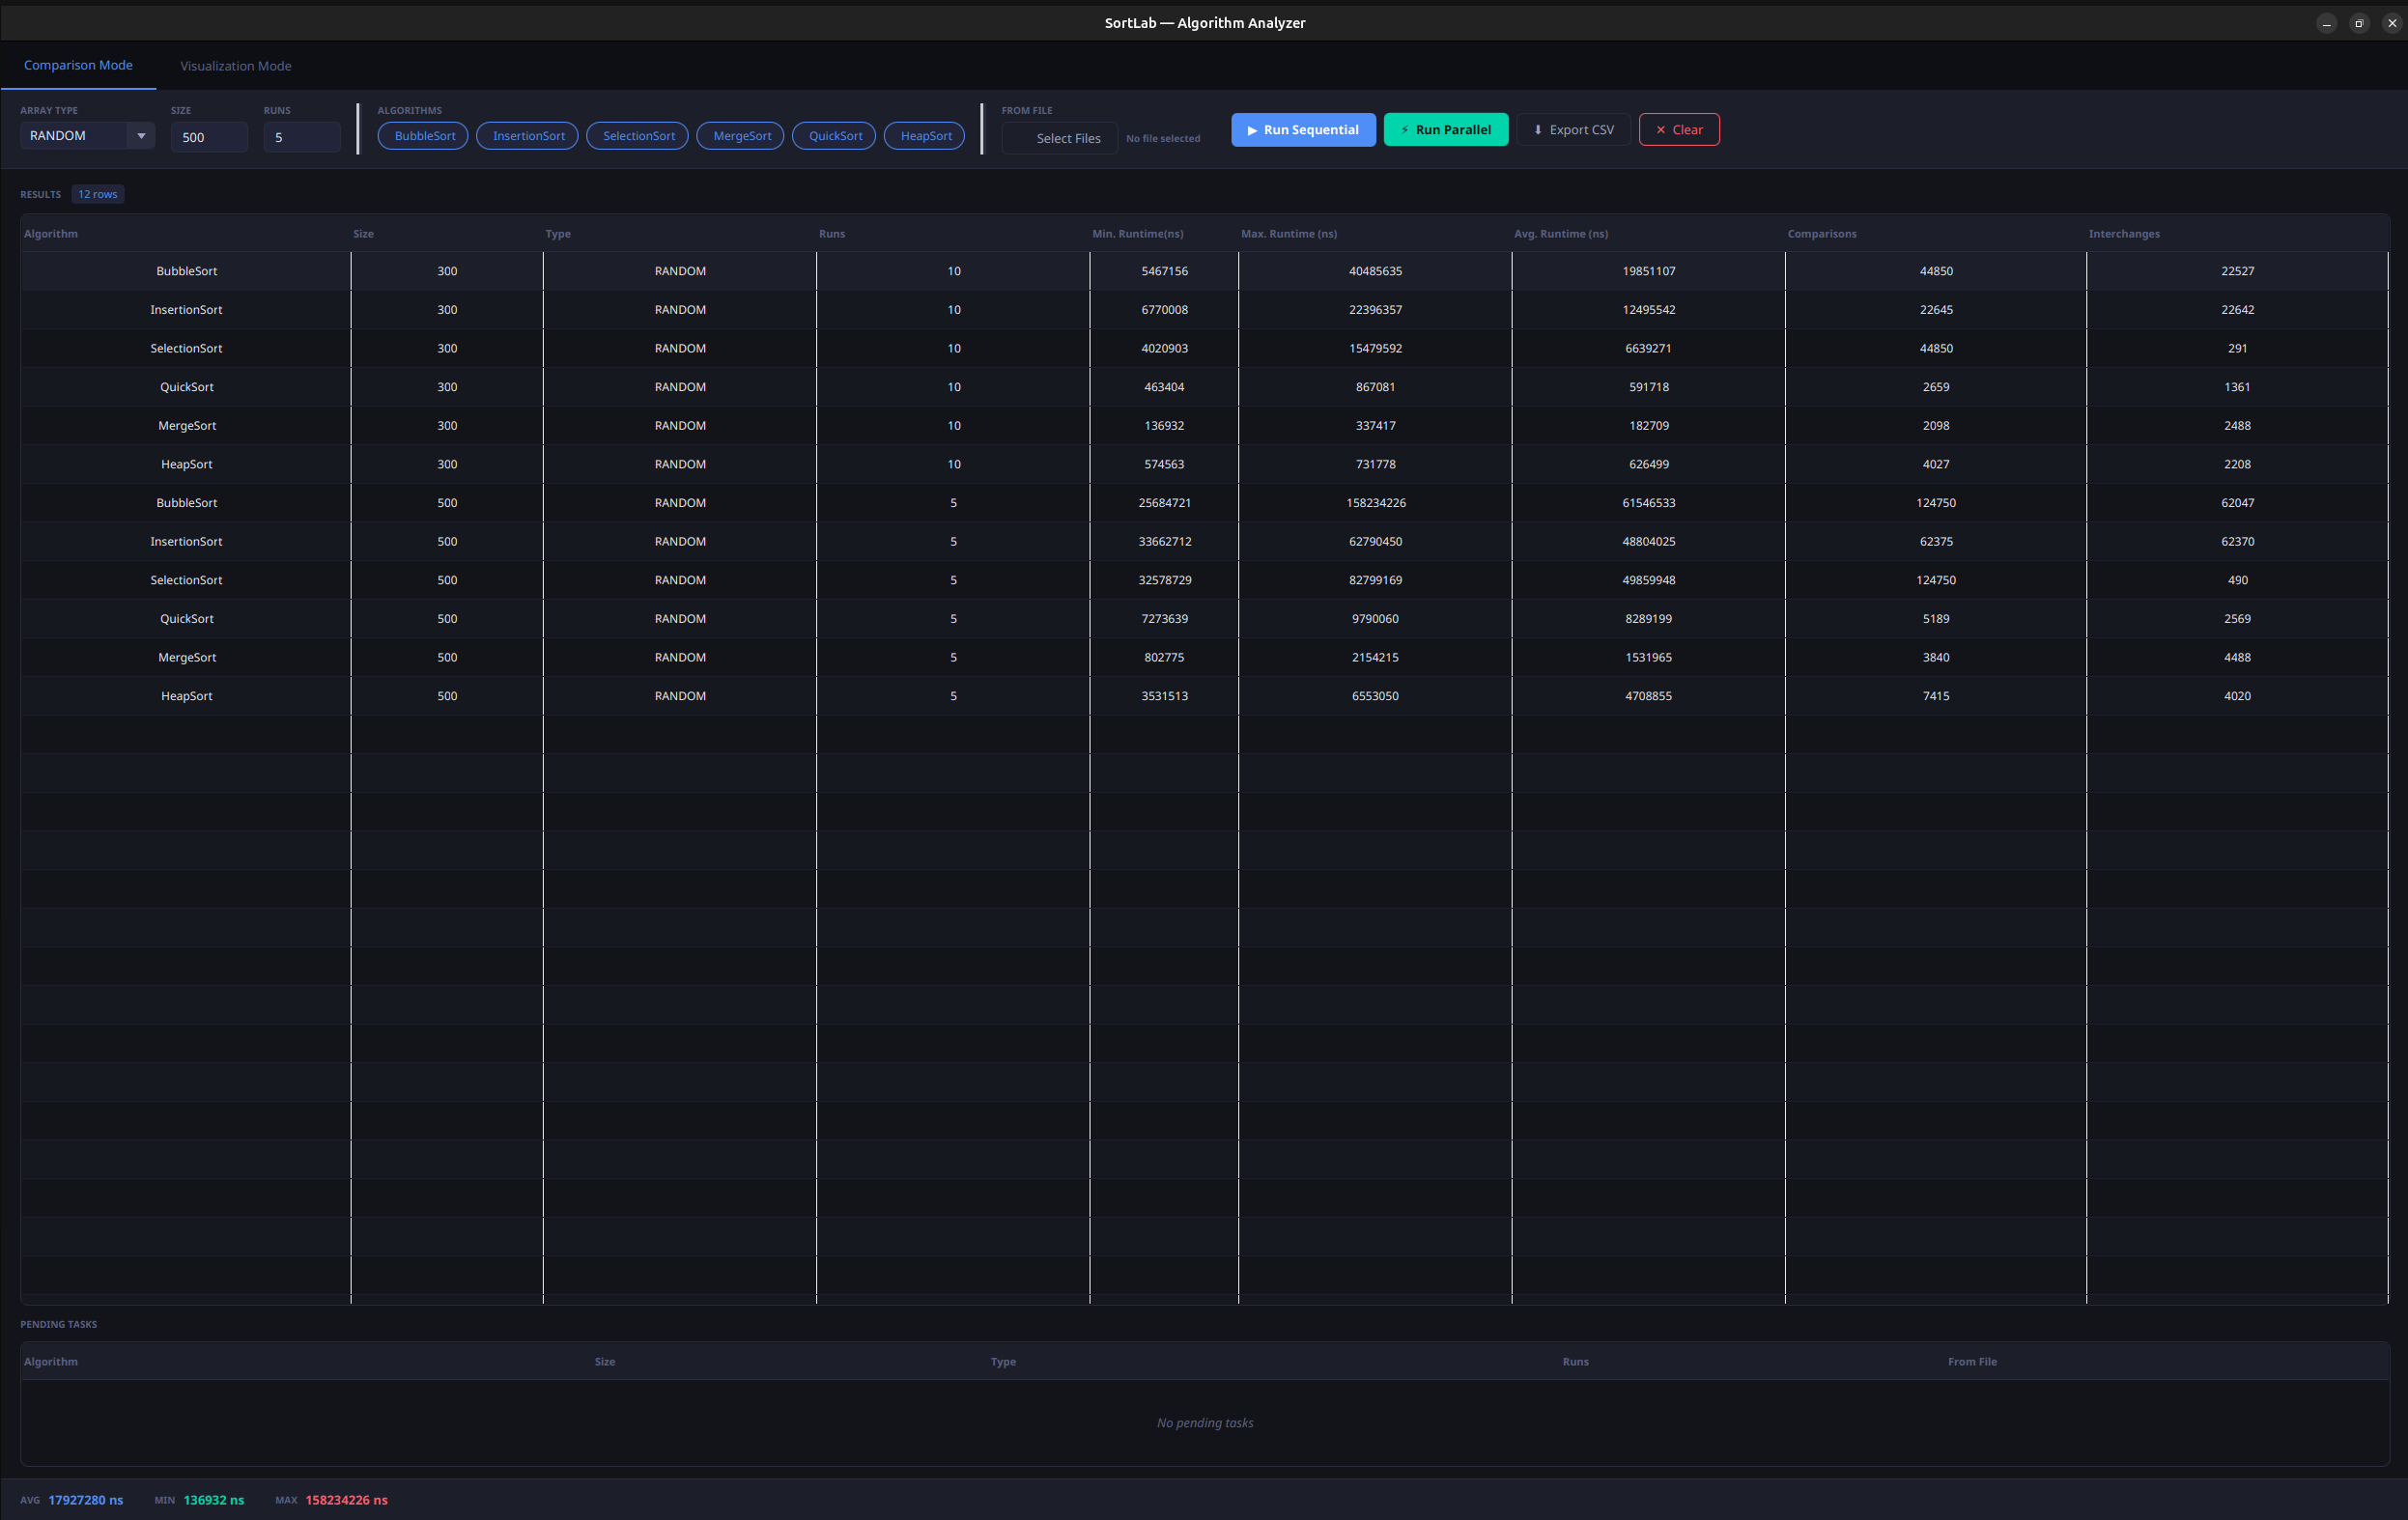
\includegraphics[width=\linewidth]{Images/comparison.png}
    \caption{Caption here}
\end{figure}

The Comparison Mode UI is a single \texttt{VBox} containing:

\begin{enumerate}[nosep]
    \item \textbf{Control Bar} (\texttt{HBox}) — Array Type combo, Size field,
          Runs field, algorithm chip-checkboxes, From File button, and action
          buttons (Run Sequential, Run Parallel, Export CSV, Clear).
    \item \textbf{Results Table} — a \texttt{TableView<ComparisonSummary>}
          with nine columns including Comparisons and Interchanges.
    \item \textbf{Pending Tasks Table} — shows tasks queued but not yet
          executed.
    \item \textbf{Summary Bar} — live Avg / Min / Max across all visible results.
\end{enumerate}

Algorithm selection uses pill-shaped \texttt{CheckBox} nodes styled with the
\texttt{.algo-chip} CSS class, which suppresses the native checkbox mark and
uses border colour changes to show selected state.

\subsection{Visualization Mode}

\begin{figure}[H]
    \centering
    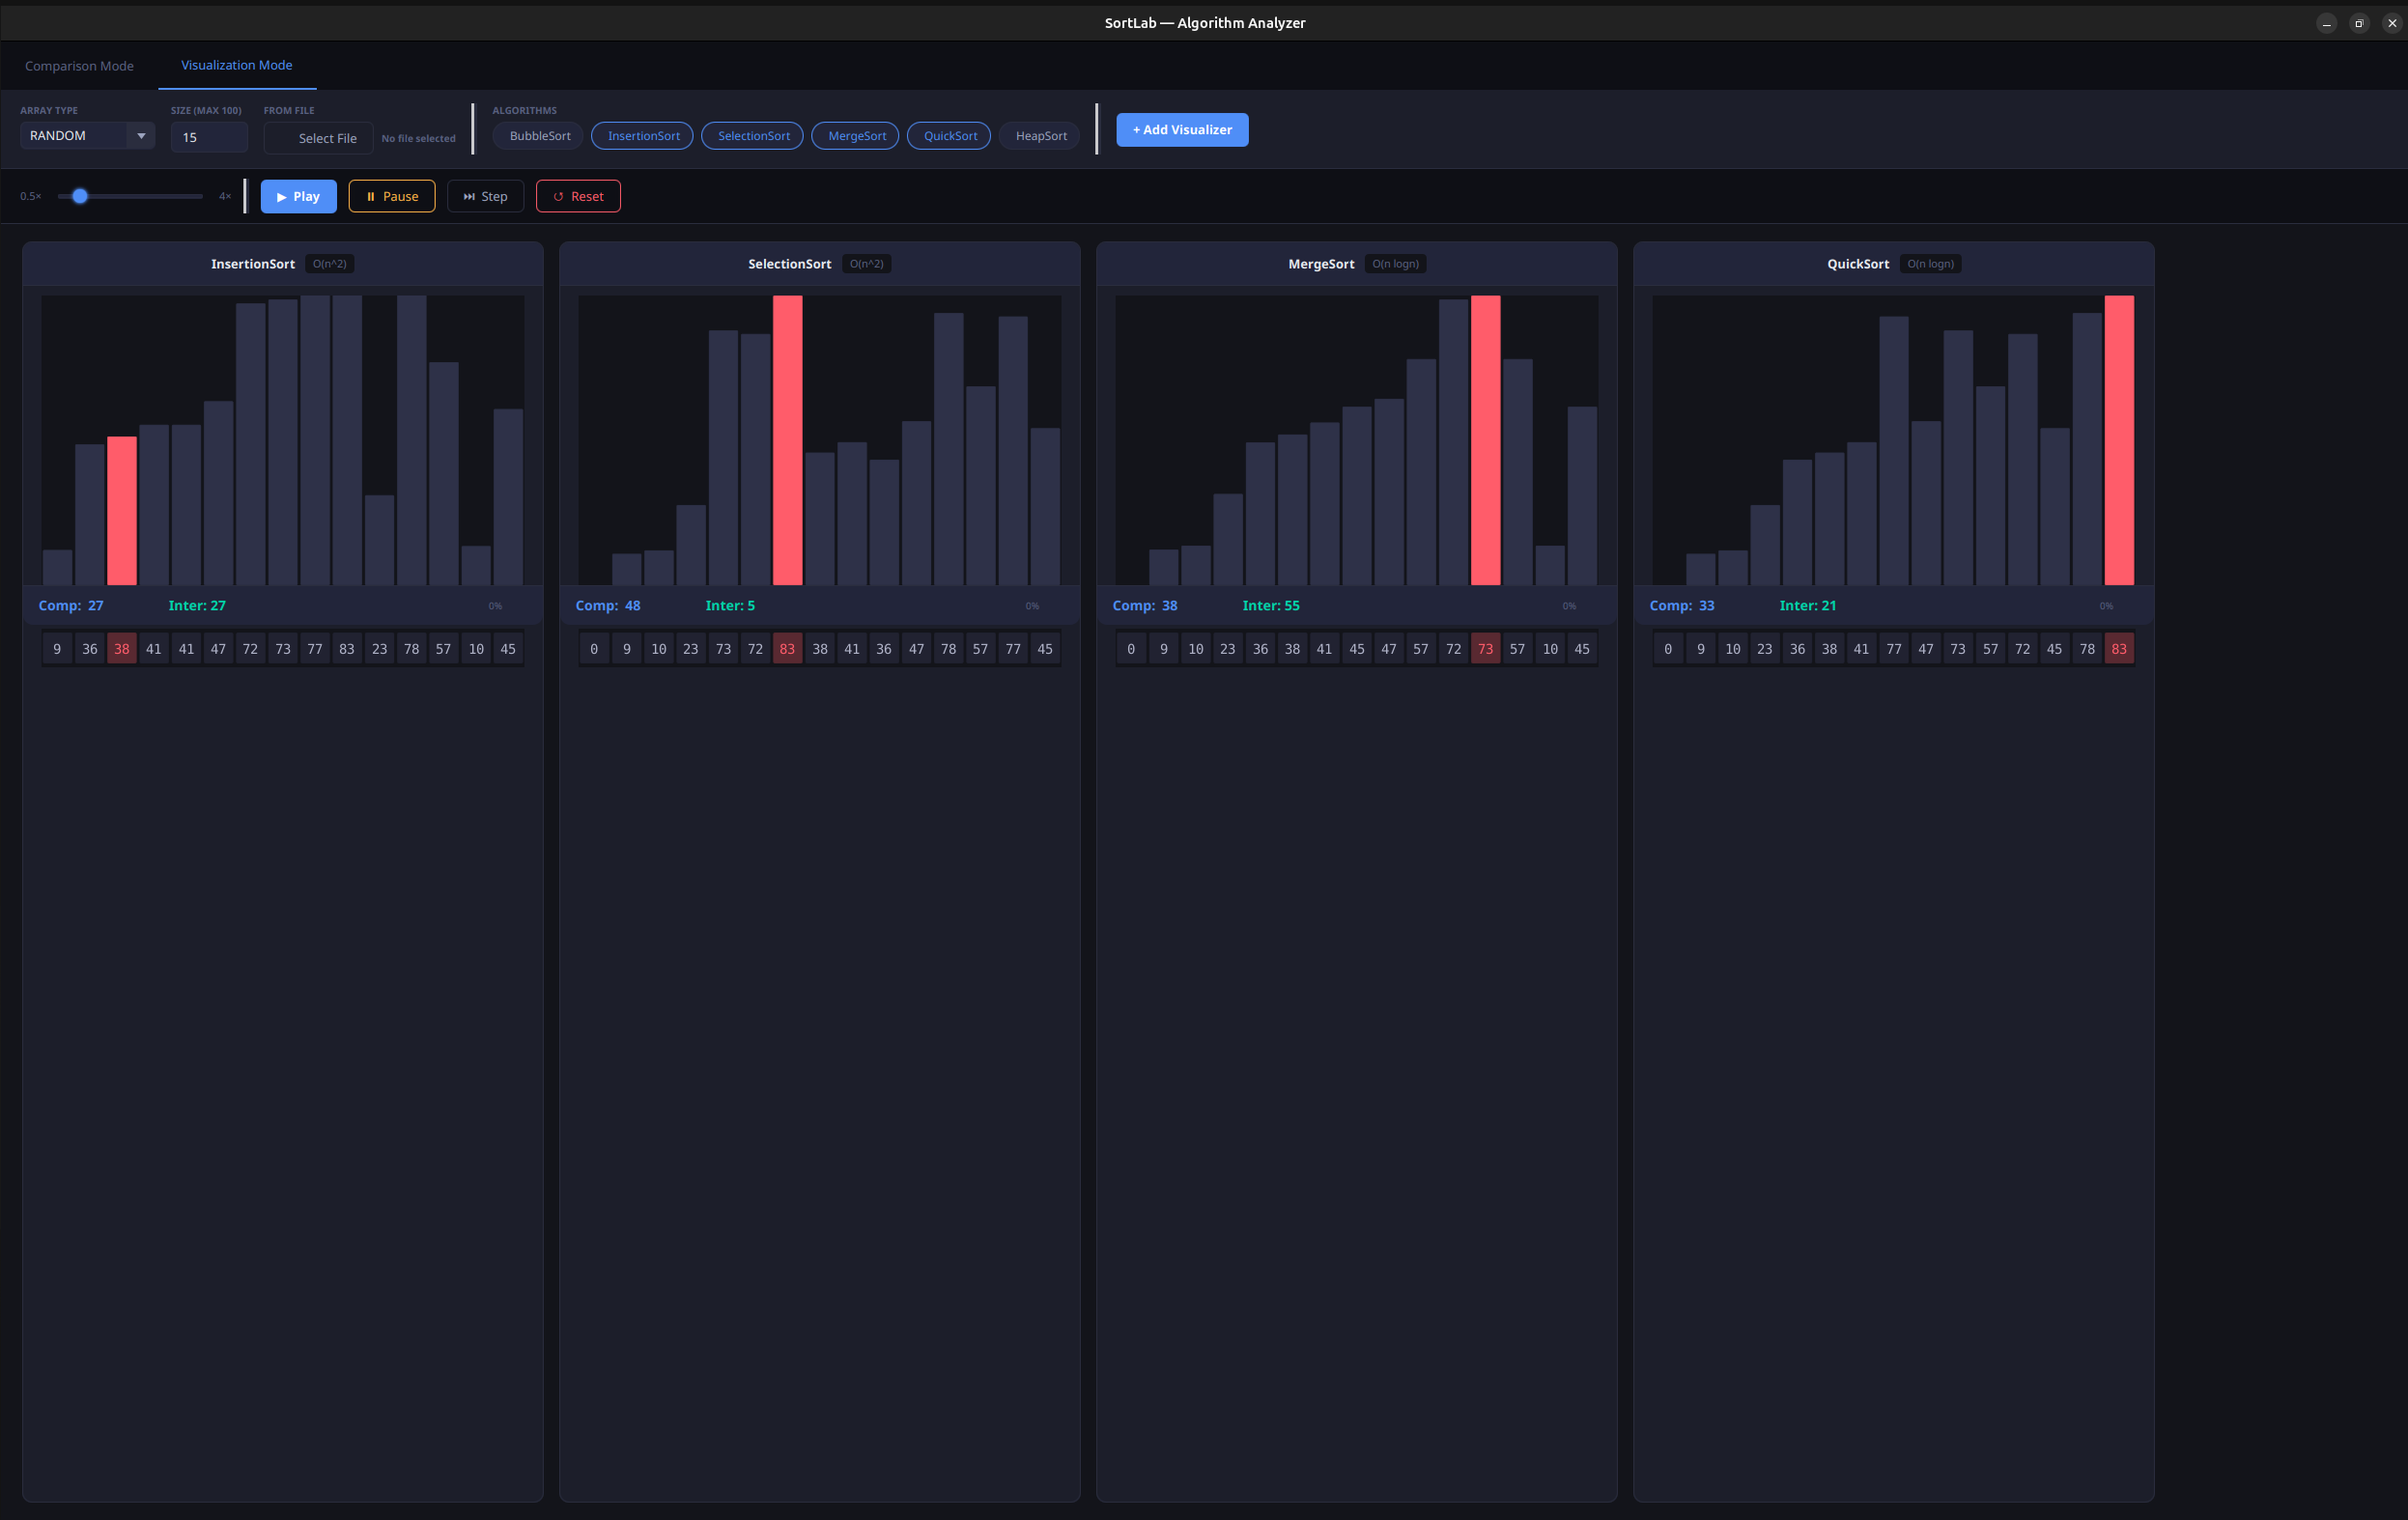
\includegraphics[width=\linewidth]{Images/visualization_start.png}
    \caption{Caption here}
\end{figure}

The Visualization Mode contains:

\begin{enumerate}[nosep]
    \item \textbf{Control Bar} — Array Type, Size, From File picker,
          algorithm chips, and ``+ Add Visualizer'' button.
    \item \textbf{Playback Bar} — speed slider (0.5$\times$ to 4$\times$),
          Play, Pause, Step, and Reset buttons.
    \item \textbf{Horizontal Scroll Panel} — a \texttt{ScrollPane} containing
          an \texttt{HBox} into which \texttt{BarChartPane} panels are appended
          at runtime. Panels scroll horizontally when more algorithms are added
          than fit on screen.
\end{enumerate}

\begin{figure}[H]
    \centering
    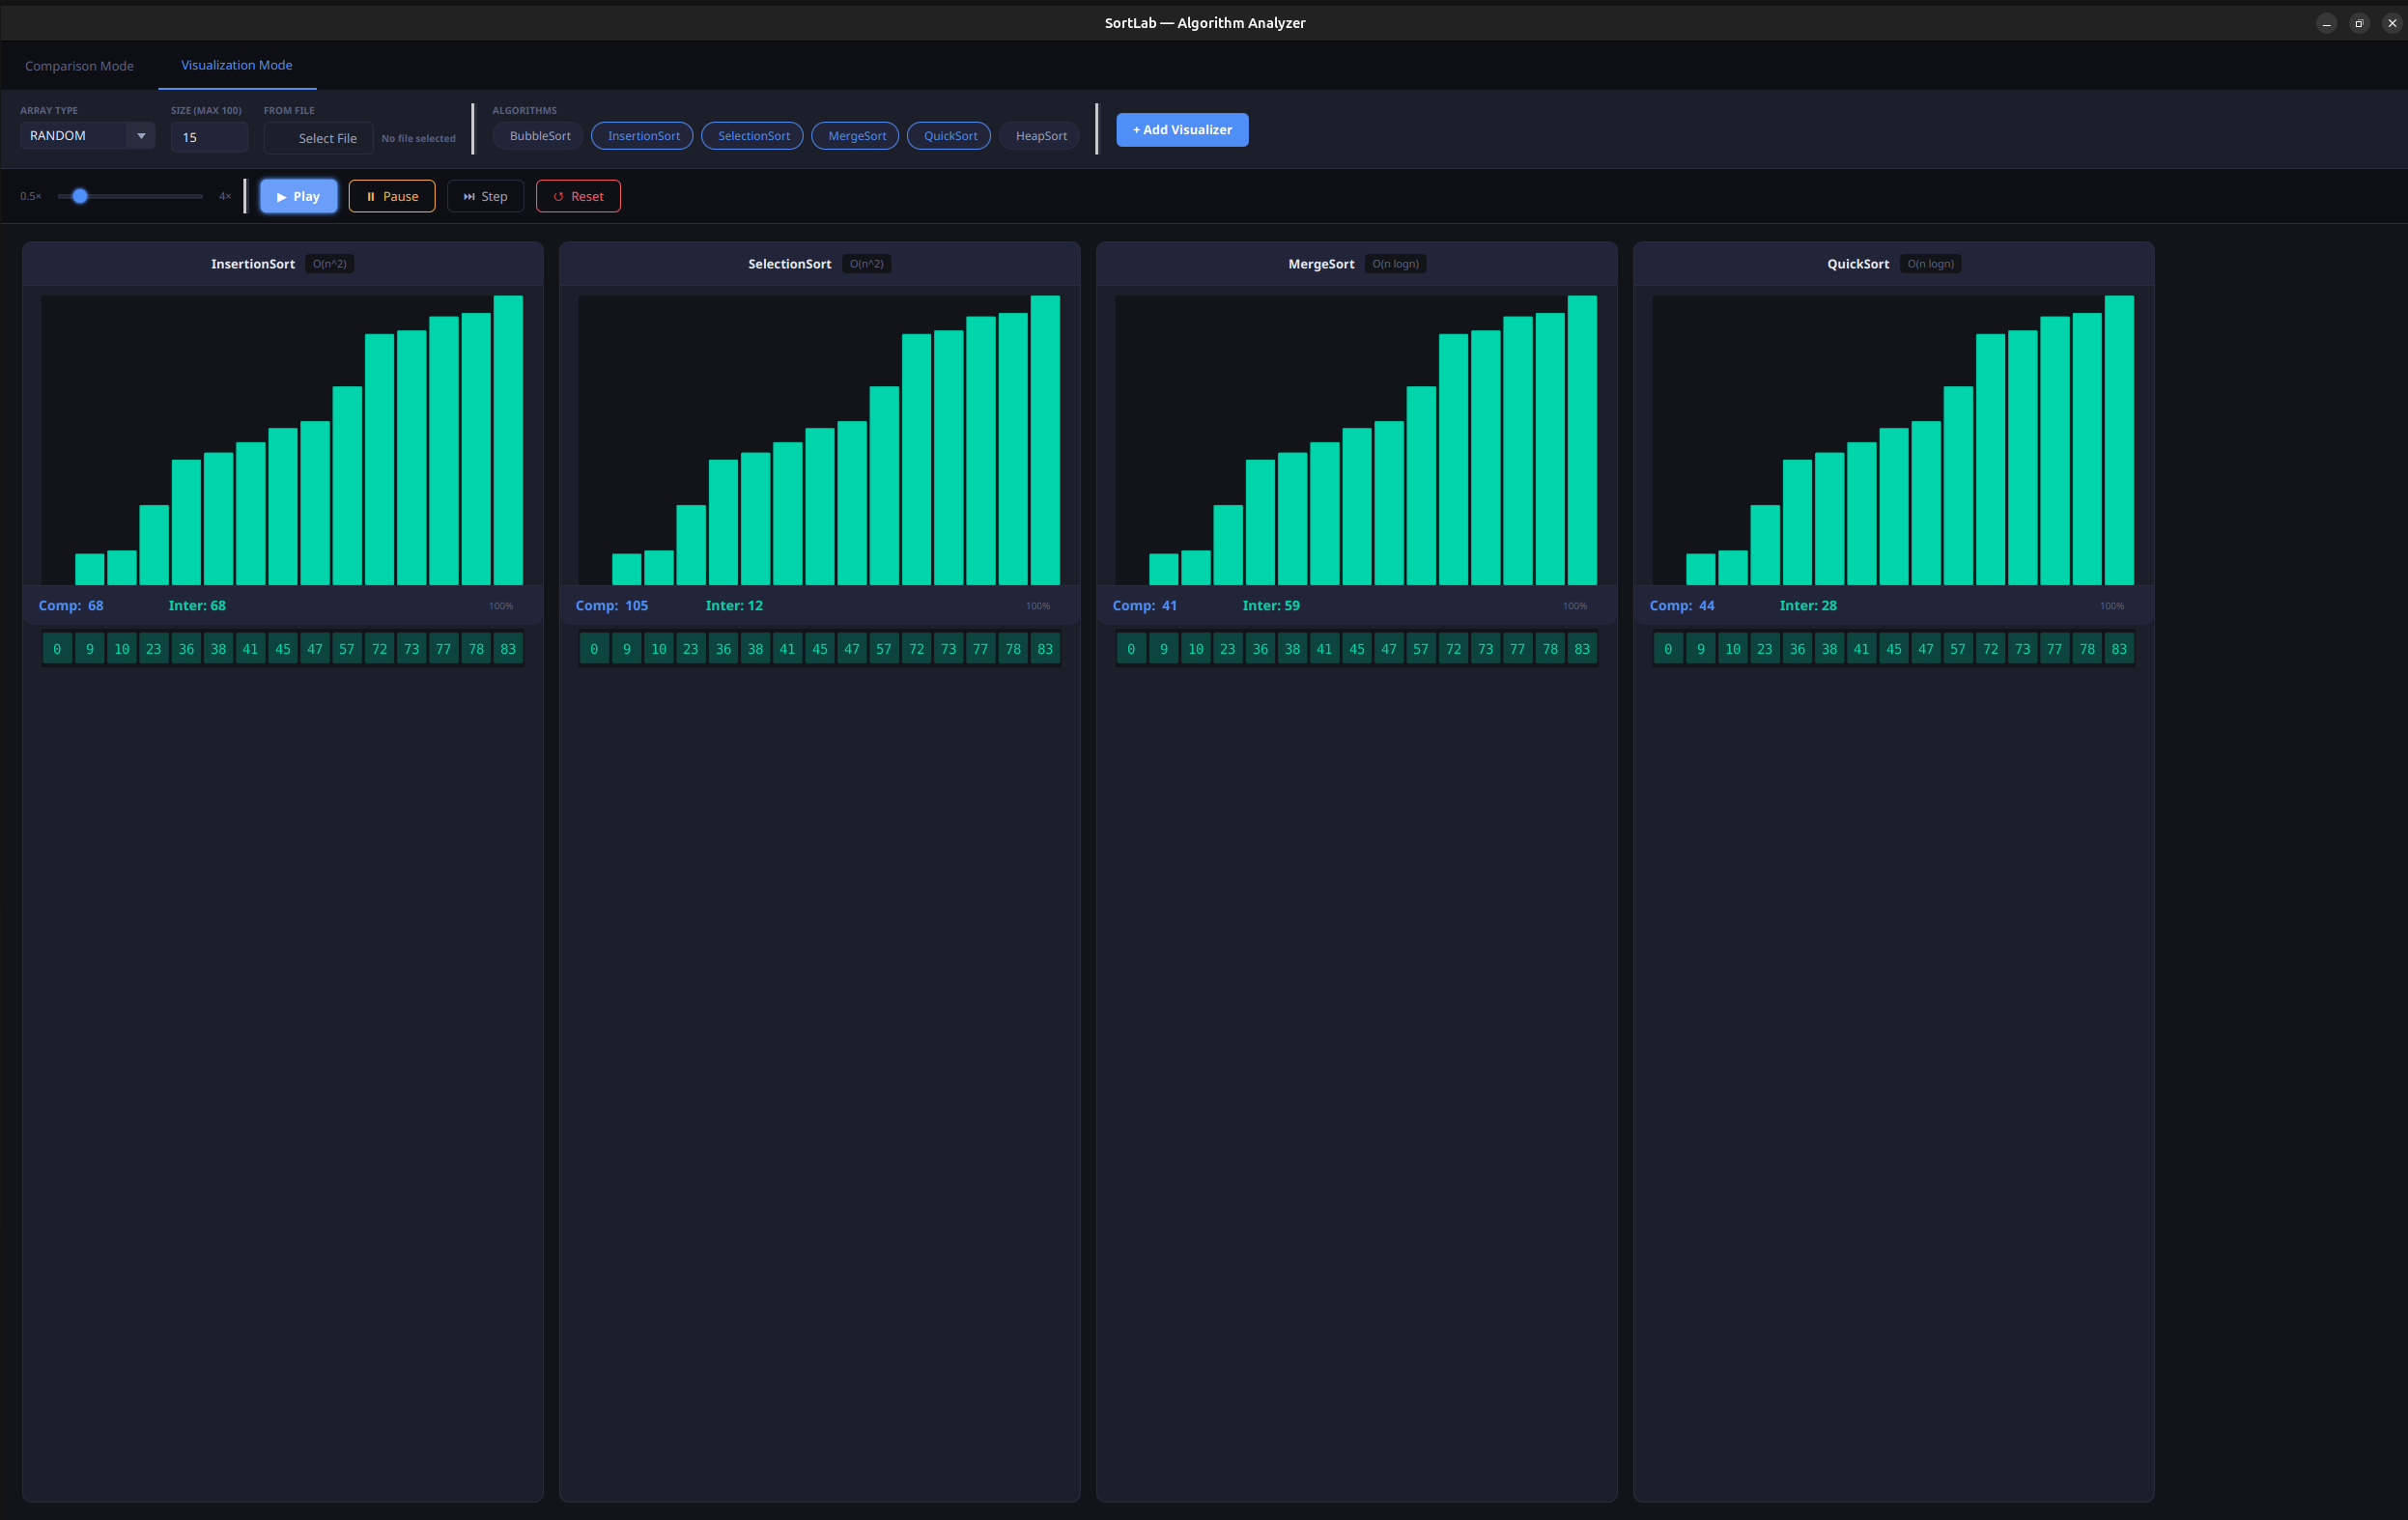
\includegraphics[width=\linewidth]{Images/visualization_end.png}
    \caption{Caption here}
\end{figure}

\subsection{UI/UX Decisions}

\begin{itemize}
    \item \textbf{Horizontal control bar:} keeps algorithm chips and settings
          on a single row so the maximum vertical space is reserved for results
          and visualizations.
    \item \textbf{Pill checkboxes:} more compact than a list of checkboxes and
          visually consistent with modern developer tool UIs.
    \item \textbf{\texttt{CONSTRAINED\_RESIZE\_POLICY\_FLEX\_LAST\_COLUMN}:}
          applied to both tables so columns fill the full width without
          horizontal scrollbars.
    \item \textbf{Live streaming results:} in Sequential mode, each
          \texttt{ComparisonSummary} is added to the table via
          \texttt{Platform.runLater()} as soon as its algorithm finishes,
          rather than waiting for all algorithms to complete.
    \item \textbf{Progress percentage:} calculated as
          $\lfloor(\text{currentStep}/\text{totalSteps}) \times 100\rfloor$
          and displayed in the stats bar of each panel.
\end{itemize}

% ══════════════════════════════════════════════════════════════════
\section{Sorting Comparison Output \& Analysis}
% ══════════════════════════════════════════════════════════════════

\subsection{Collected Data}

The table below shows a representative sample from the \texttt{results.csv} file,
collected using the Comparison Mode with RANDOM input type across three array sizes
(100, 300, 400 elements) and varying run counts:

\begin{center}
\scriptsize
\begin{longtable}{lrrlrrrr}
\toprule
\textbf{Algorithm} & \textbf{Size} & \textbf{Runs} & \textbf{Type} &
\textbf{Avg (ns)} & \textbf{Min (ns)} & \textbf{Max (ns)} &
\textbf{Comp.} \\
\midrule
BubbleSort    & 100 & 100 & RANDOM & 750,467   & 352,211  & 5,803,687 & 4,950 \\
InsertionSort & 100 & 100 & RANDOM & 560,313   & 306,845  & 1,674,896 & 2,561 \\
SelectionSort & 100 & 100 & RANDOM & 528,305   & 349,855  & 1,048,928 & 4,950 \\
QuickSort     & 100 & 100 & RANDOM & 332,790   & 108,103  & 1,228,300 & 650   \\
MergeSort     & 100 & 100 & RANDOM & 61,513    & 39,790   & 176,833   & 541   \\
HeapSort      & 100 & 100 & RANDOM & 233,510   & 132,486  & 456,999   & 1,028 \\
\midrule
BubbleSort    & 300 & 50  & RANDOM & 10,185,426 & 4,993,517 & 29,965,229 & 44,850 \\
InsertionSort & 300 & 50  & RANDOM & 8,289,404  & 6,619,645 & 17,243,300 & 22,569 \\
SelectionSort & 300 & 50  & RANDOM & 8,497,681  & 5,868,859 & 21,194,684 & 44,850 \\
QuickSort     & 300 & 50  & RANDOM & 1,409,268  & 1,020,697 & 4,449,643  & 2,634  \\
MergeSort     & 300 & 50  & RANDOM & 246,827    & 188,073   & 359,762    & 2,098  \\
HeapSort      & 300 & 50  & RANDOM & 1,540,107  & 1,151,458 & 4,722,822  & 4,021  \\
\midrule
BubbleSort    & 400 & 200 & RANDOM & 22,427,551 & 11,658,736 & 69,209,992 & 79,800 \\
InsertionSort & 400 & 200 & RANDOM & 18,212,252 & 14,998,566 & 45,766,251 & 40,014 \\
SelectionSort & 400 & 200 & RANDOM & 18,251,822 & 14,258,478 & 46,555,382 & 79,800 \\
QuickSort     & 400 & 200 & RANDOM & 2,078,641  & 1,353,684  & 13,918,646 & 3,831  \\
MergeSort     & 400 & 200 & RANDOM & 583,378    & 284,707    & 11,536,066 & 2,960  \\
HeapSort      & 400 & 200 & RANDOM & 2,146,044  & 1,414,536  & 13,953,056 & 5,698  \\
\bottomrule
\end{longtable}
\end{center}

\subsection{Python Analysis Graphs}

The \texttt{analyze\_sorts.py} script reads the exported CSV and generates a
2$\times$2 grid of matplotlib plots styled to match the Carbon Dark theme.

\subsubsection{Graph 1 — Average Runtime (Log Scale)}

\begin{figure}[H]
    \centering
    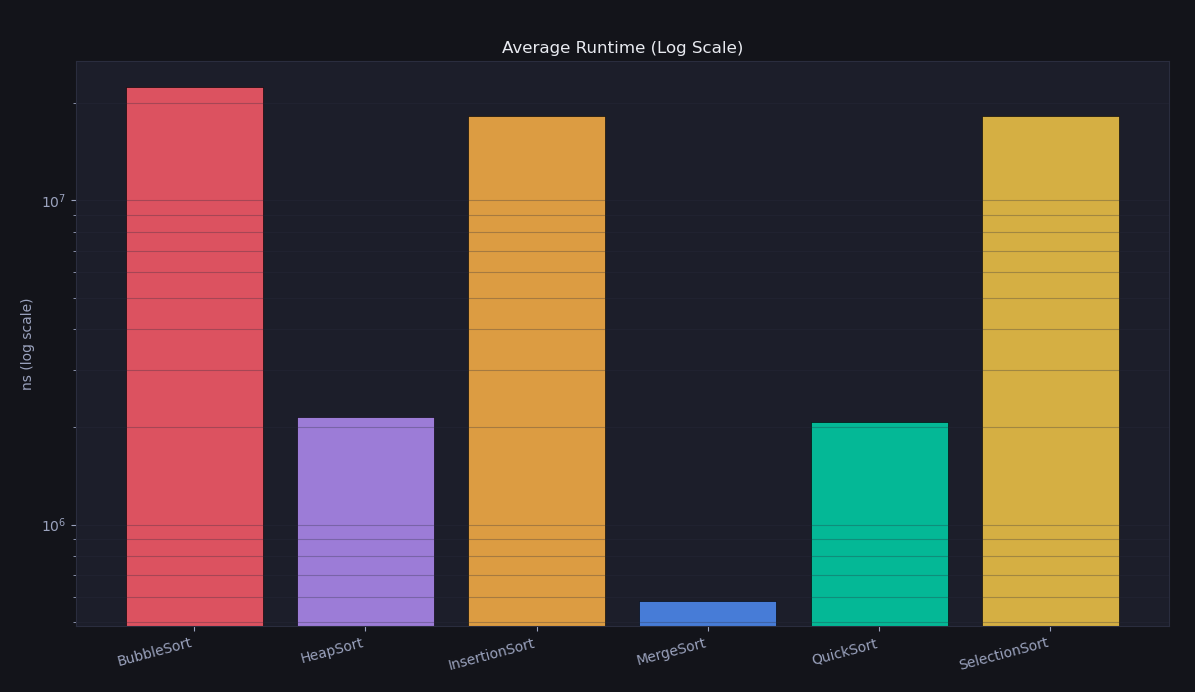
\includegraphics[width=\linewidth]{Images/runtime_avg.png}
    \caption{Caption here}
\end{figure}

This chart immediately illustrates the dramatic performance gap between the
$O(n^2)$ group (Bubble, Insertion, Selection) and the $O(n \log n)$ group
(Merge, Quick, Heap). MergeSort consistently achieves the lowest average
runtime due to predictable memory access patterns and guaranteed
$O(n \log n)$ behaviour. Log scale is essential here because the
$O(n^2)$ algorithms are 10--40$\times$ slower than the $O(n \log n)$ ones,
and a linear scale would compress the fast algorithms to near-zero bars.

\subsubsection{Graph 2 — Min / Avg / Max Runtime (Log Scale)}

\begin{figure}[H]
    \centering
    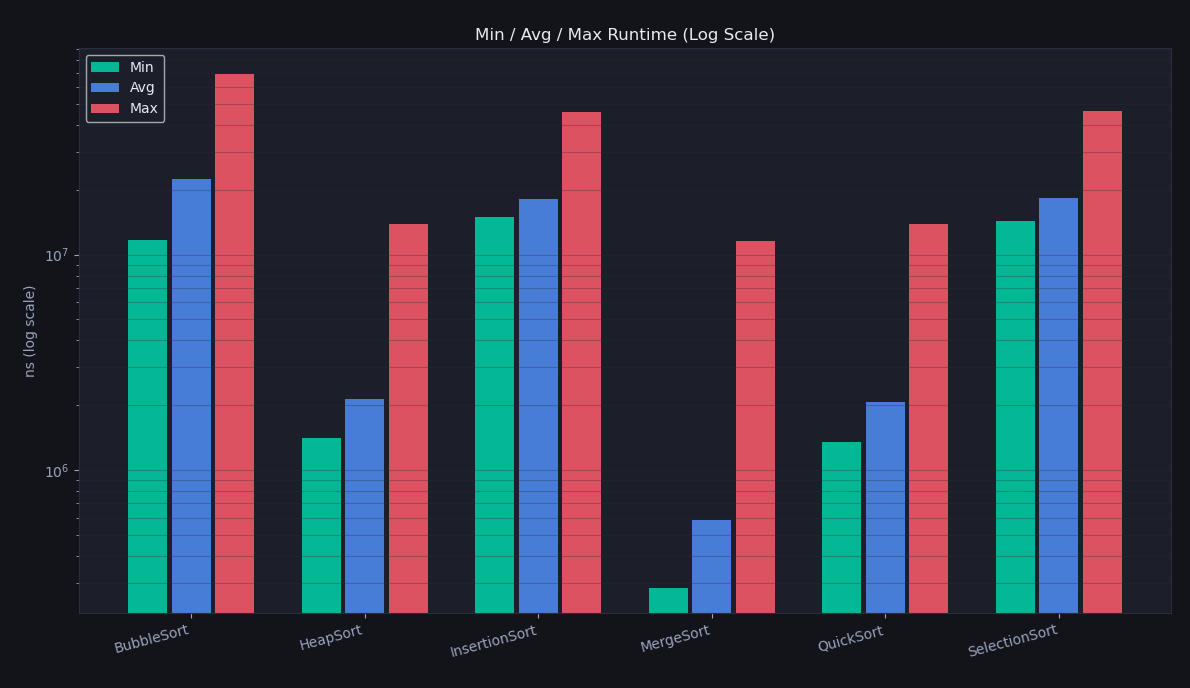
\includegraphics[width=\linewidth]{Images/runtime_stats.png}
    \caption{Caption here}
\end{figure}

The spread between Min and Max reveals algorithm \emph{consistency}:

\begin{itemize}
    \item \textbf{MergeSort:} very tight spread — always $O(n \log n)$,
          little variation.
    \item \textbf{QuickSort:} wider spread — randomised pivot occasionally
          produces poor partitioning.
    \item \textbf{BubbleSort:} wide spread — heavily influenced by OS
          scheduling since it spends so long sorting.
\end{itemize}

\subsubsection{Graph 3 — Comparisons vs Interchanges}

\begin{figure}[H]
    \centering
    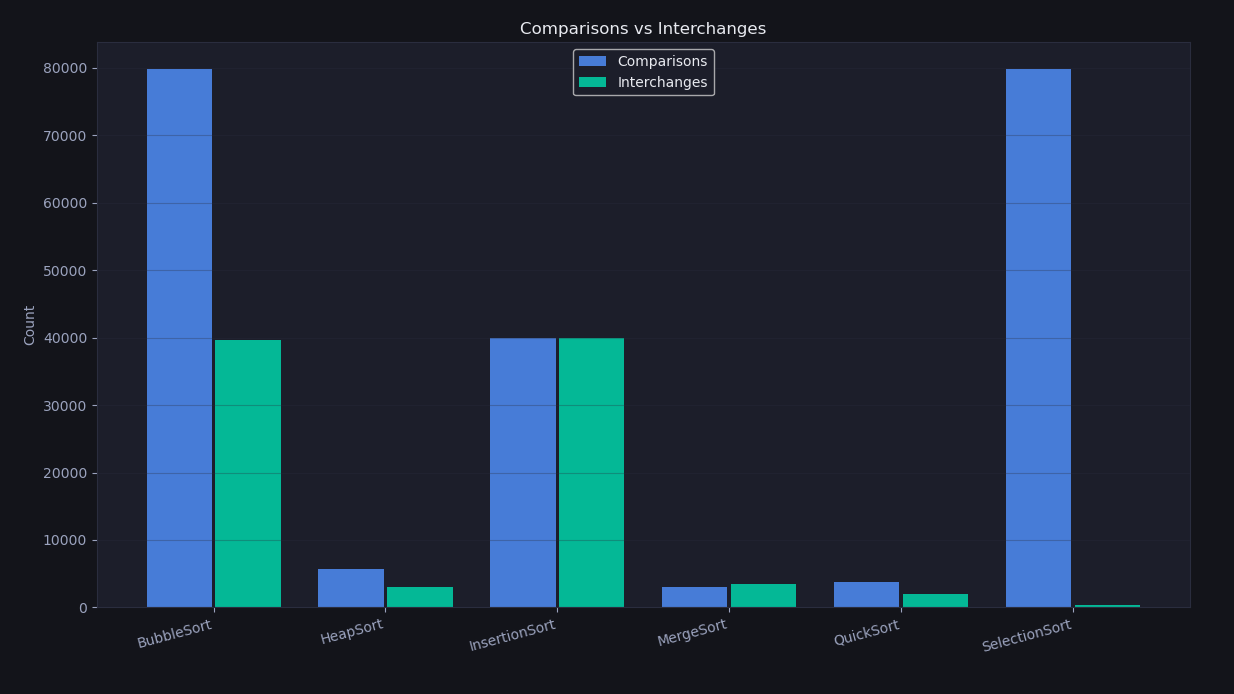
\includegraphics[width=\linewidth]{Images/comparisons_interchanges.png}
    \caption{Caption here}
\end{figure}

Key observations from the Comparisons vs Interchanges chart:

\begin{itemize}
    \item \textbf{SelectionSort:} highest comparisons ($\frac{n(n-1)}{2}$)
          but fewest interchanges ($n-1$). It is comparison-heavy but
          swap-efficient.
    \item \textbf{MergeSort:} fewest comparisons despite $O(n \log n)$ —
          because each comparison directly decides a placement.
    \item \textbf{InsertionSort:} comparisons $\approx$ interchanges because
          every shift is counted as an interchange, and each shift is paired
          with a comparison that triggered it.
\end{itemize}

\subsubsection{Graph 4 — Runtime Scaling}

\begin{figure}[H]
    \centering
    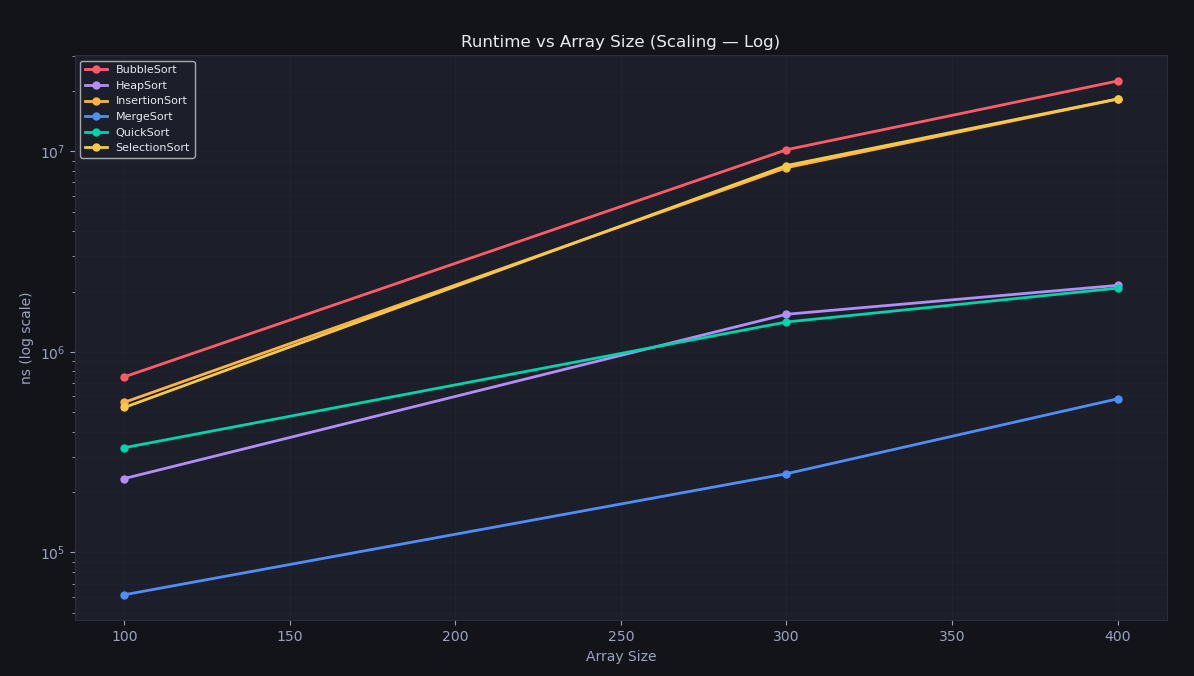
\includegraphics[width=\linewidth]{Images/runtime_scaling.png}
    \caption{Caption here}
\end{figure}

The scaling chart is the most powerful visualisation of algorithmic complexity.
On a log-scale y-axis:
\begin{itemize}
    \item $O(n \log n)$ algorithms appear nearly linear (gradual climb).
    \item $O(n^2)$ algorithms show a much steeper curve.
    \item The divergence between the two groups becomes strikingly clear at
          sizes above 300 elements.
\end{itemize}

\subsection{Analysis Interpretation}

\begin{center}
\begin{tabular}{lcccc}
\toprule
\textbf{Algorithm} & \textbf{Speed Rank} & \textbf{Consistency} &
\textbf{Comparisons} & \textbf{Interchanges} \\
\midrule
MergeSort     & 1\textsuperscript{st} & Very High & Low     & Medium \\
QuickSort     & 2\textsuperscript{nd} & High      & Low     & Low    \\
HeapSort      & 3\textsuperscript{rd} & High      & Medium  & Medium \\
SelectionSort & 4\textsuperscript{th} & Medium    & Very High & Very Low \\
InsertionSort & 5\textsuperscript{th} & Medium    & Medium  & High   \\
BubbleSort    & 6\textsuperscript{th} & Low       & Very High & High   \\
\bottomrule
\end{tabular}
\end{center}

MergeSort is the fastest in all benchmark runs due to its guaranteed
$O(n \log n)$ behaviour and efficient memory access pattern during the merge
phase. QuickSort closely follows and would likely outperform MergeSort in
cache-sensitive environments because it is an in-place algorithm. BubbleSort
performs worst in every metric: highest comparisons, high interchanges, and
the greatest variance between runs.

% ══════════════════════════════════════════════════════════════════
\section{Visualization Mode Output}
% ══════════════════════════════════════════════════════════════════

\subsection{Panel Anatomy}

Each algorithm panel in Visualization Mode contains the following visual regions:

\begin{enumerate}
    \item \textbf{Header:} Algorithm name (bold, white) and complexity
          (\texttt{O(n\textsuperscript{2})} or \texttt{O(n log n)}) in a
          grey badge — fixed, never changes.
    \item \textbf{Bar Chart:} Up to 100 vertical bars, colour-coded:
    \begin{itemize}[nosep]
        \item \textcolor{danger}{\textbf{Red}} (\texttt{\#ff5c6a}) — currently
              active element being compared.
        \item \textcolor{muted}{\textbf{Dark grey}} (\texttt{\#2e3148}) —
              idle elements.
        \item \textcolor{accent}{\textbf{Teal}} (\texttt{\#00d4aa}) — all
              elements once sorting completes.
    \end{itemize}
    \item \textbf{Stats Bar:} Live Comparisons count (blue), Interchanges
          count (teal), and progress percentage — all update every frame.
    \item \textbf{Array Box Row:} One box per element below the bars, showing
          the integer value. Font size adapts from 14px down to 7px as array
          size increases. Boxes below 10px width hide their text label.
\end{enumerate}

\begin{figure}[H]
    \centering
    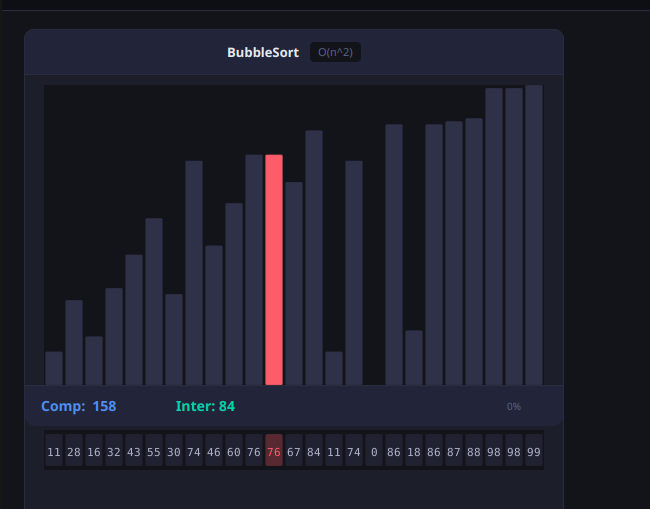
\includegraphics[width=\linewidth]{Images/bubblesort_running.png}
    \caption{Caption here}
\end{figure}

\begin{figure}[H]
    \centering
    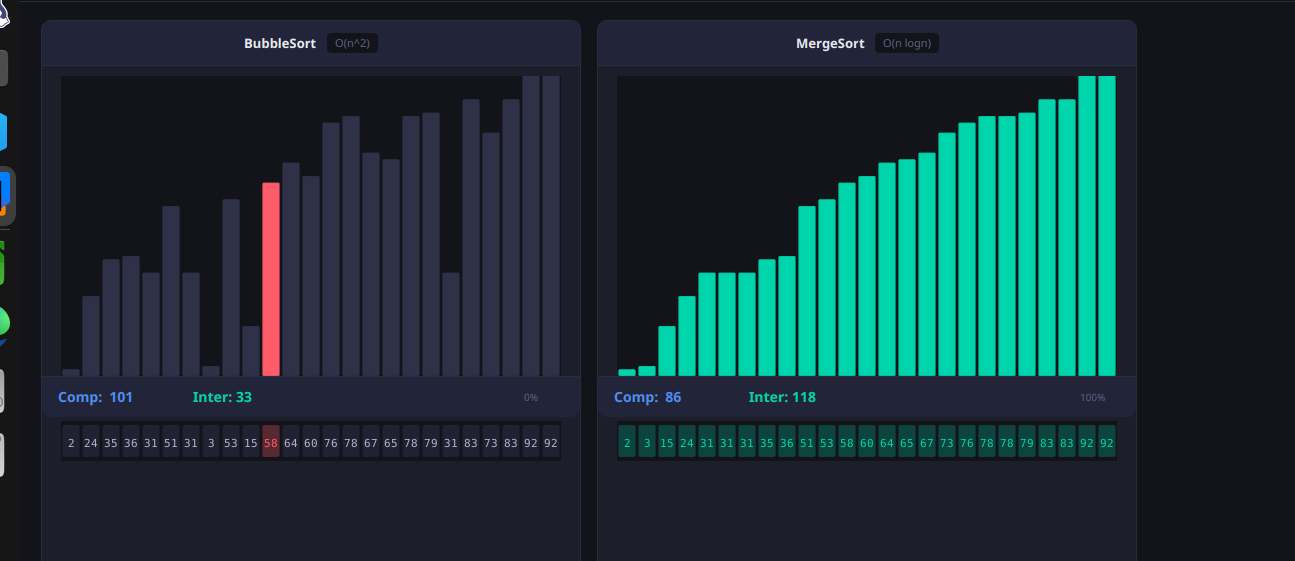
\includegraphics[width=\linewidth]{Images/bubble_vs_merge.png}
    \caption{Caption here}
\end{figure}
\subsection{Audio Feedback}

The \texttt{Audio} class generates real-time tones synchronised to the currently
active bar. A single persistent \texttt{SourceDataLine} is opened once and
reused across all frames (via \texttt{ensureAudioLine()}) to avoid the latency
of creating a new audio line each frame.

The pitch is proportional to bar height:
\[
f = 150 + \frac{\text{value}}{\text{maxValue}} \times 1050 \quad \text{Hz}
\]

Each tone is 50ms, with a 10\% fade-in envelope and 20\% fade-out envelope
applied to eliminate audible clicks at tone boundaries. This technique is known
as an ``attack/release'' envelope in audio engineering. The volume is kept at
30\% to avoid being intrusive.

\subsection{Animation Speed Control}

The speed slider maps $[0.5, 4.0] \to$ delay in milliseconds:

\[
\text{delayMs} = \frac{300}{\text{speed}}
\]

\begin{center}
\begin{tabular}{lrr}
\toprule
\textbf{Slider Setting} & \textbf{Delay (ms)} & \textbf{FPS (approx.)} \\
\midrule
0.5$\times$ (slowest) & 600 ms & 1.7 fps \\
1.0$\times$ (default) & 300 ms & 3.3 fps \\
2.0$\times$           & 150 ms & 6.7 fps \\
4.0$\times$ (fastest) & 75 ms  & 13.3 fps \\
\bottomrule
\end{tabular}
\end{center}

% ══════════════════════════════════════════════════════════════════
\section{Input \& File Handling}
% ══════════════════════════════════════════════════════════════════

\subsection{Random Generation}

\texttt{ArrayGenerator.generateFromRandom(int size, ArrayType type)} creates an
array of random integers in $[0, 100)$ and then:

\begin{itemize}[nosep]
    \item \texttt{RANDOM} — returns as-is.
    \item \texttt{SORTED} — applies \texttt{Arrays.sort()}.
    \item \texttt{INVERSELY\_SORTED} — sorts then reverses the array in-place
          using a manual two-pointer swap loop.
\end{itemize}

\subsection{File Input Format}

Input files must contain a single line in the format:

\begin{center}
\texttt{[5, 1, 2, 6, 4, 8, 12, 0]}
\end{center}

The parser strips \texttt{[} and \texttt{]} characters, splits on
\texttt{", "}, and parses each token as an integer.
Visualization Mode enforces a 100-element maximum and a 2-element minimum.

\begin{figure}[H]
    \centering
    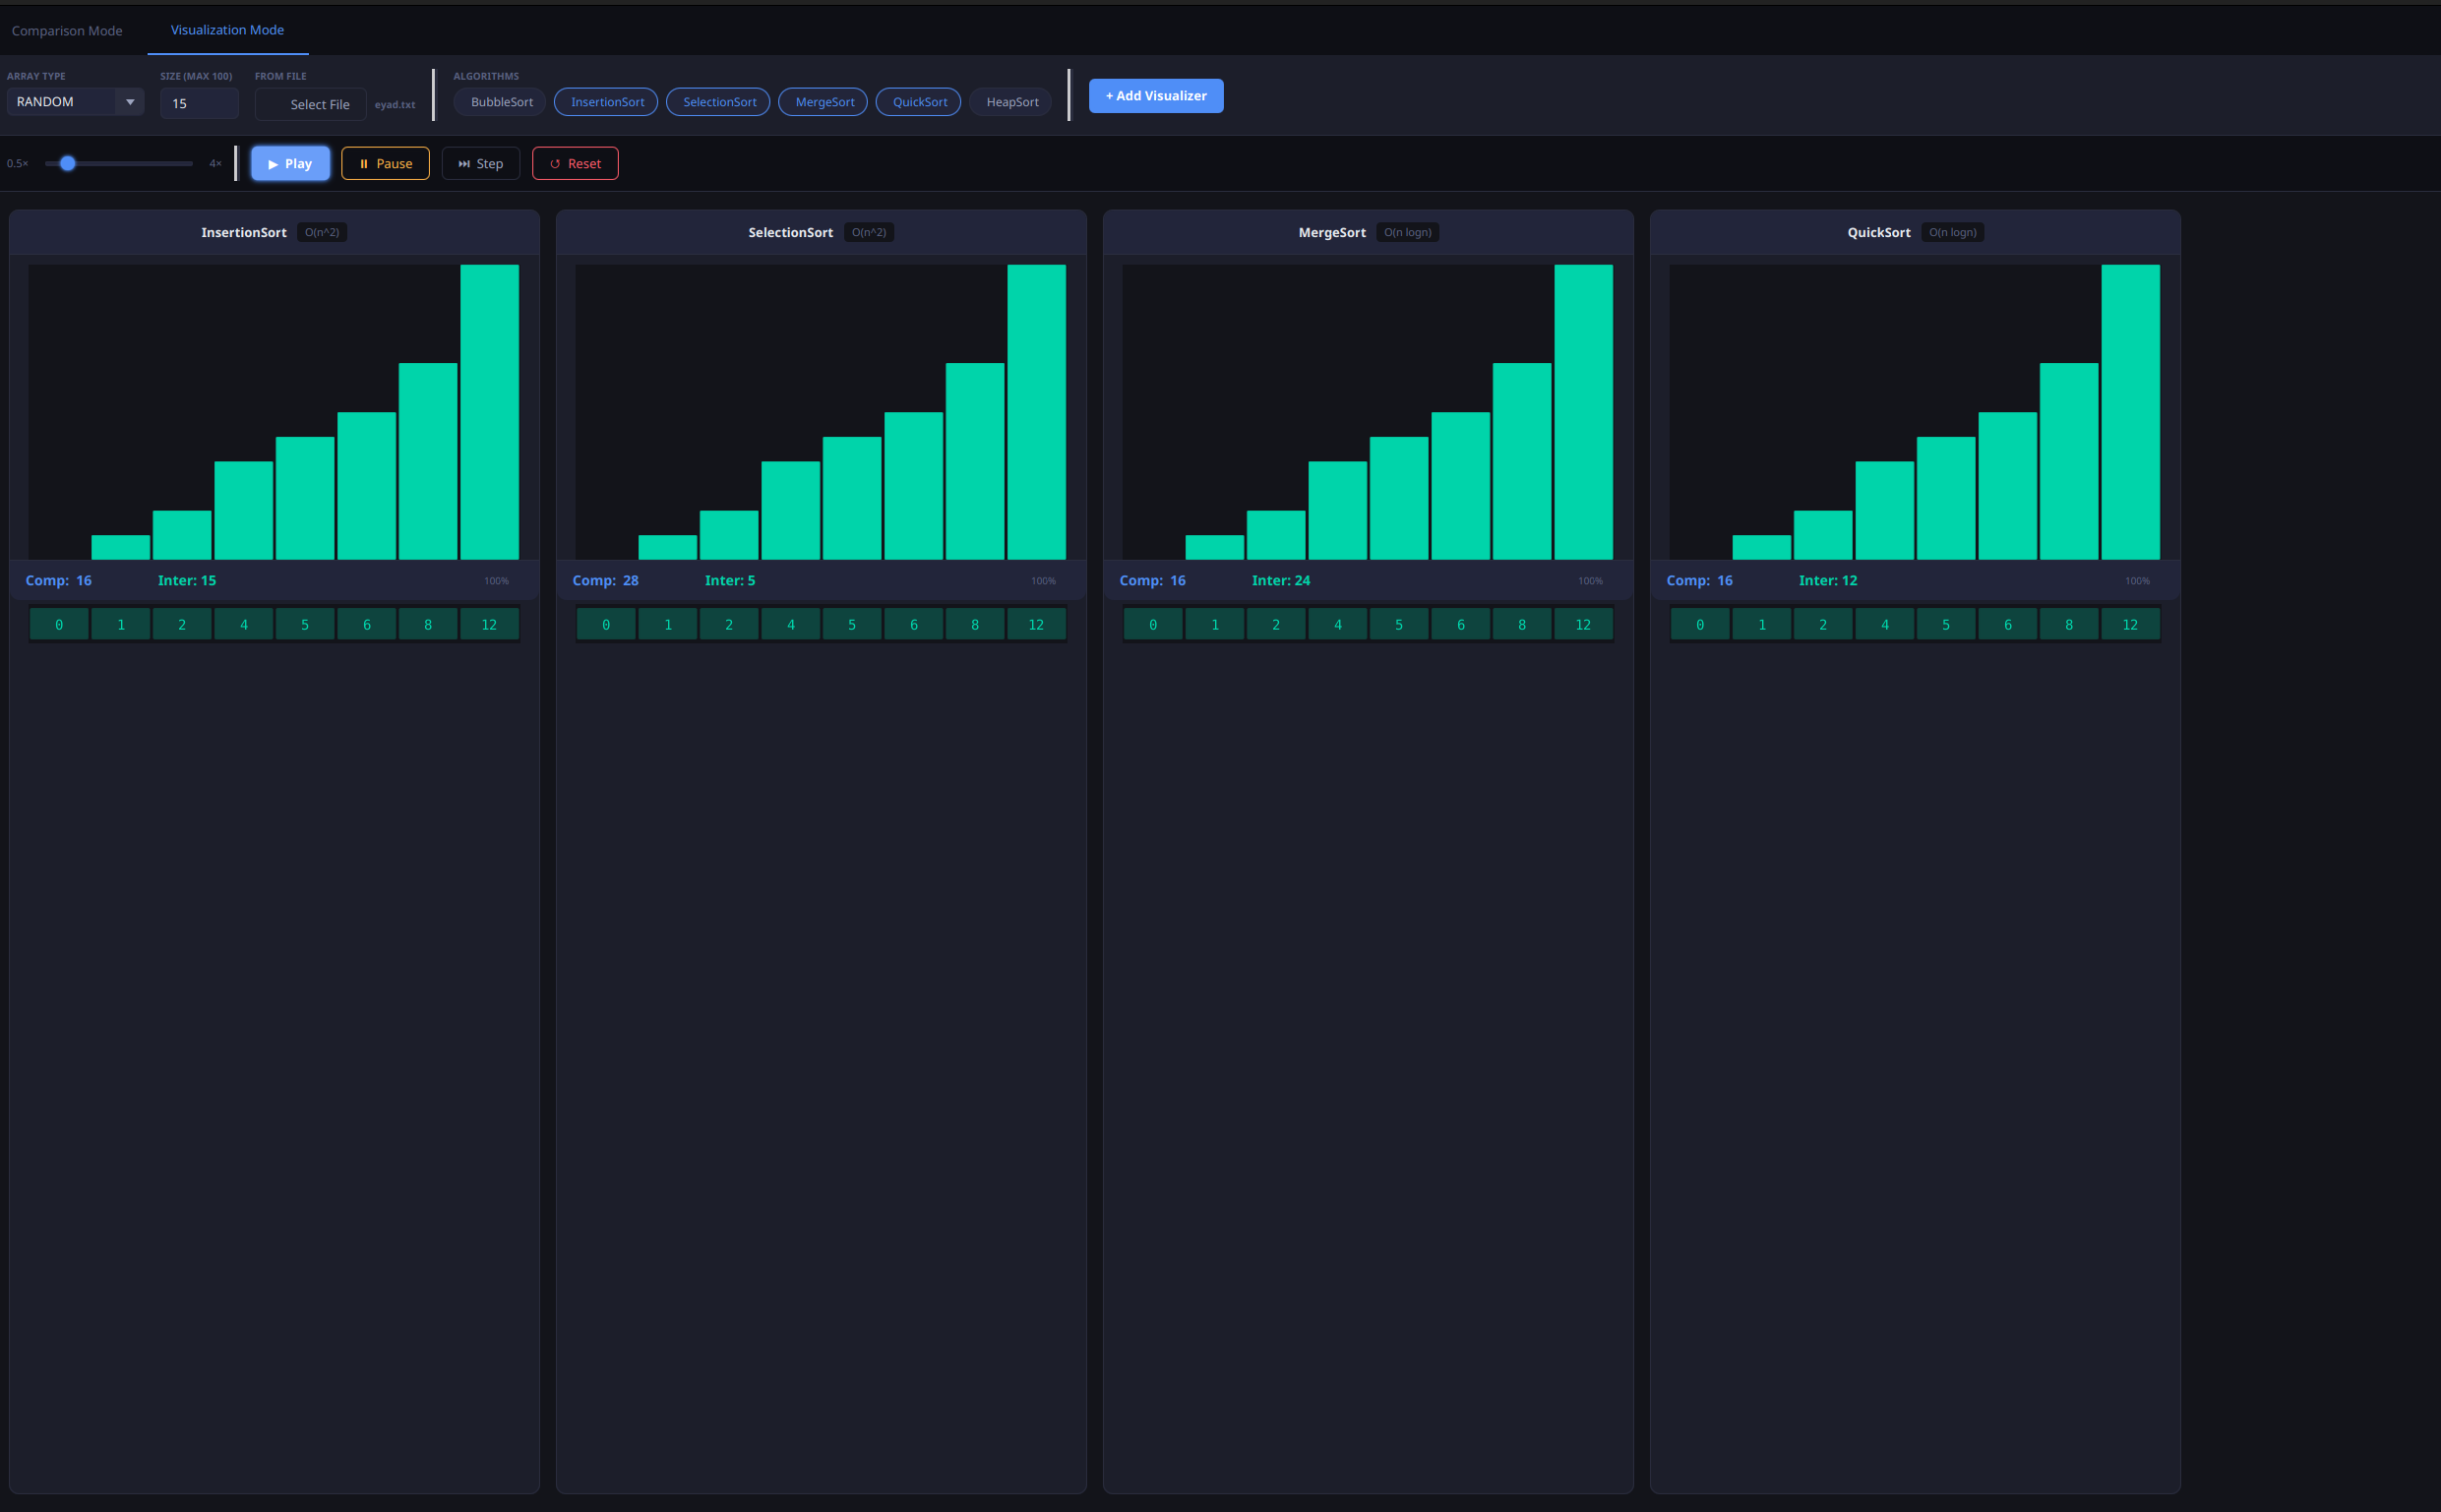
\includegraphics[width=\linewidth]{Images/visualization_final.png}
    \caption{Caption here}
\end{figure}

% ══════════════════════════════════════════════════════════════════
\section{Concurrency Design}
% ══════════════════════════════════════════════════════════════════

The application uses two layers of threading:

\subsection{Background Tasks (JavaFX \texttt{Task})}

Both \texttt{handleRunSequential()} and \texttt{handleRunParallel()} in
\texttt{ComparisonController} wrap their work in a JavaFX \texttt{Task<Void>}
launched on a plain \texttt{Thread}. This prevents the sort benchmarks from
blocking the JavaFX Application Thread (which would freeze the UI). Results are
pushed back to the UI via \texttt{Platform.runLater()}.

\subsection{Parallel Comparison (\texttt{ExecutorService})}

\texttt{ParallelComparisonManager} submits each \texttt{ComparisonTask} to a
fixed thread pool, allowing multiple algorithms to be benchmarked simultaneously:

\begin{lstlisting}[caption={Parallel task submission}]
executor = Executors.newFixedThreadPool(
    Math.min(tasks.size(),
             Runtime.getRuntime().availableProcessors())
);
for (ComparisonTask task : tasks) {
    Future<List<SortResult>> future = executor.submit(() -> {
        ComparisonRunner runner = new ComparisonRunner(task);
        return runner.run();
    });
    futures.add(future);
}
\end{lstlisting}

The pool size is capped at the number of CPU cores to avoid over-subscription
(creating more threads than the CPU can run simultaneously would introduce
context-switching overhead that degrades benchmark accuracy).

\subsection{Audio Threading}

The \texttt{Audio.playTone()} method is called on the JavaFX Application Thread
from within \texttt{drawFrame()}, but the audio write itself (\texttt{audioLine.write()})
is synchronised on \texttt{audioLock} and executed inline. This is acceptable
because the audio buffer is small (50ms at 44100 Hz = $\sim$4400 samples)
and the write is fast enough not to cause visible frame drops.

% ══════════════════════════════════════════════════════════════════
\section{Build \& Run}
% ══════════════════════════════════════════════════════════════════

\subsection{Prerequisites}

\begin{itemize}[nosep]
    \item Java 21 (JDK)
    \item Maven 3.8+
    \item Python 3.10+ with \texttt{pandas}, \texttt{matplotlib},
          \texttt{numpy} (for analysis script)
\end{itemize}

\subsection{Running the Application}

\begin{lstlisting}[language=bash, style=pythonstyle,
                   caption={Build and run commands}]
# From the SortingAlgorithms/ directory:
mvn clean javafx:run

# Or build and run the JAR:
mvn clean package
java -jar target/SortingAlgorithms-1.0.jar
\end{lstlisting}

\subsection{Running the Python Analysis}

\begin{lstlisting}[language=bash, style=pythonstyle,
                   caption={Analysis script usage}]
cd SortingAlgorithms
source venv/bin/activate
python3 analyze_sorts.py data/output/results.csv
\end{lstlisting}

% ══════════════════════════════════════════════════════════════════
\section{Conclusion}
% ══════════════════════════════════════════════════════════════════

SortLab successfully delivers a comprehensive platform for studying sorting
algorithms through both quantitative benchmarking and qualitative visualisation.

The key findings from the benchmark data are:

\begin{enumerate}
    \item \textbf{MergeSort} is the fastest algorithm across all tested sizes,
          with the most consistent performance (lowest Min-to-Max spread).
    \item \textbf{QuickSort} achieves comparable speed to MergeSort and uses
          less memory (in-place), though its randomised pivot introduces more
          variance.
    \item \textbf{HeapSort} provides guaranteed $O(n \log n)$ like MergeSort
          but is approximately 3--4$\times$ slower in practice due to poor
          cache locality (heap accesses jump around memory rather than
          sequentially).
    \item The \textbf{$O(n^2)$ group} (Bubble, Insertion, Selection) degrades
          rapidly with size. At $n=400$ they are 10--40$\times$ slower than
          the $O(n \log n)$ group.
    \item \textbf{SelectionSort} makes far fewer swaps than BubbleSort or
          InsertionSort but makes the same number of comparisons as BubbleSort,
          making it useful when write operations are expensive.
\end{enumerate}

The visualisation component makes these differences tangible — watching MergeSort
finish in seconds while BubbleSort is still on its third pass over the same
array gives an intuition that no table of numbers can fully convey.

\end{document}